\documentclass{article}

% if you need to pass options to natbib, use, e.g.:
%     \PassOptionsToPackage{numbers, compress}{natbib}
% before loading neurips_2018

% ready for submission
%\usepackage{neurips_2018}

% to compile a preprint version, e.g., for submission to arXiv, add add the
% [preprint] option:
\usepackage[preprint]{neurips_2018}

% to compile a camera-ready version, add the [final] option, e.g.:
% \usepackage[final]{neurips_2018}

% to avoid loading the natbib package, add option nonatbib:
%     \usepackage[nonatbib]{neurips_2018}

\usepackage[utf8]{inputenc} % allow utf-8 input
\usepackage[T1]{fontenc}    % use 8-bit T1 fonts
\usepackage{url}            % simple URL typesetting
\usepackage{booktabs}       % professional-quality tables
\usepackage{amsfonts}       % blackboard math symbols
\usepackage{nicefrac}       % compact symbols for 1/2, etc.
\usepackage{microtype}      % microtypography
\usepackage{hyperref} % <====================== last packge to be called
\usepackage{graphicx}
\hypersetup{linkbordercolor=green}

\title{Sentiment Analysis for Movie Reviews}

% The \author macro works with any number of authors. There are two commands
% used to separate the names and addresses of multiple authors: \And and \AND.
%
% Using \And between authors leaves it to LaTeX to determine where to break the
% lines. Using \AND forces a line break at that point. So, if LaTeX puts 3 of 4
% authors names on the first line, and the last on the second line, try using
% \AND instead of \And before the third author name.

\author{%
  Jiachen Ning \ Linhong Li \ Shiqi Xiao \ Xiangting Chen \\
  % 
  Carnegie Mellon University\\
  Pittsburgh, PA 15213 \\
  % Address \\
  % \texttt{email} \\
  % \AND
  % Coauthor \\
  % Affiliation \\
  % Address \\
  % \texttt{email} \\
  % \And
  % Coauthor \\
  % Affiliation \\
  % Address \\
  % \texttt{email} \\
  % \And
  % Coauthor \\
  % Affiliation \\
  % Address \\
  % \texttt{email} \\
}

\begin{document}
% \nipsfinalcopy is no longer used

\maketitle

\section{Introduction}

Sentiment Analysis is the task of classifying text documents by their {\it sentiment}, or the overall opinion towards the subject matter \cite{Pang}. In practice, sentiment analysis is useful for companies and policymakers to monitor large scale public opinions on specific products and/or policies, and thus extended applications of sentiment analysis can be found in security, medical, finance, and entertainment domains \cite{Mantyl}.

The goal of this project is to build an interpretable sentiment classifier based not only on text content information, but also on lexical polarity information and unobserved topic information that could be derived from the text, using one of the most analyzed dataset for sentiment analysis -- the IMDb Dataset of movie reviews. The dataset contains a collection of 50,000 reviews posted on the Internet Movie Database. Standard preprocessing ensured that the dataset is balanced, containing the same number of positive and negative reviews, where positive reviews had a score greater than or equal to 7 and negative reviews had a score less than or equal to 4 \cite{Mass}. 

Our primary task is to output a binary classification of an audience's attitude towards a movie based on his or her online review. To do that, we will experiment with both content-based and topic-based input representations of the movie reviews on a variety of classification models. The performance of our model will be evaluated based on classification accuracy.



\section{Literature Review}

Literature review suggested that successful sentiment analysis requires finding (1) the most representative text embeddings and (2) the best performing classification scheme. 

For the first requirement, it is a standard practice to tokenize the text into sequences of n words, called n-gram representations, with bigram and trigram representations being the most widely used and showing superior results than unigram tokens \cite{Wang}. To vectorize a tokenized text, common methods include counting the token occurrences (i.e., Bag-of-Word, or BoW model) and assigning a term frequency (TF) or term frequency-inverse document frequency (TF-IDF) score to each token in the corpus dictionary, both of which reflect how important a token is to a document. However, the BoW and TF-IDF models are based solely on the text content. The joint sentiment/topic model proposed by Lin and He suggested that unsupervised topic modeling techniques such as LDA could potentially lead to more informative feature text representation for sentiment analysis \cite{Lin}. Besides topic information, it was shown that weighting words by their lexical polarity and part of speech improves classification accuracy. 


In terms of the second requirement for a successful sentiment analysis, several common choices of classifiers presented in previous works include Na{\"i}ve Bayes (NB), Support Vector Machine(SVM), and (Deep) Neural Networks (NN) \cite{Howard, Wang} . For the IMDB dataset, the current best classifier is ULMFiT, which is a LSTM-based model proposed by Howard and Ruder in 2018 \cite{Howard}; SVM with NB features (NBSVM) proposed by Wang and Mannings showed superior performance among non-NN classifiers \cite{Wang}.


\section{Methods}

Currently, most existing works mainly focused on testing various classifiers on content-based feature vectors. Thus, we explored different combinations of feature vectorization (BoW, TF, and TF-IDF) and the two most effective classifiers used in sentiment analysis, NB and SVM. For the SVM model, we used both linear and RBF kernels. Note that we fixed the tokenization to be unigram and bigram since it tends to give better performance \cite{Pang}. All baseline models are constructed, trained, and tested using the machine learning package, scikit-learn \cite{Pedregosa}.




\section{Preliminary Results}

The combination of different vectorization methods and classifiers, as well as their respective testing prediction accuracies are given in Table~\ref{tab:a} and Figure~$\ref{fig:a}$.

\begin{table}[h]
   \centering
  \begin{tabular}{ l l|| c | c | c} 
     \toprule
    Tokenization  & Vectorization & NB & SVM-Linear & SVM-RBF  \\

    \midrule
    Unigram  & BoW  & 0.81968   & 0.83212      & -        \\
    Uni + Bi & BoW  & 0.84272    & 0.87504       & 0.63148          \\
    Uni + Bi + Tri & BoW  & 0.84476  & 0.83212      & -       \\
    Unigram  & TF  & 0.84308    & 0.87560      & -    \\
    Uni + Bi & TF & 0.85372     & 0.88060       & 0.67400      \\
    Uni + Bi + Tri & TF  & 0.85336  & 0.88092     & -     \\
    Unigram  & TF-IDF  & 0.83128    & 0.87240      & -    \\
    Uni + Bi & TF-IDF  & 0.85476      & 0.88584       & 0.65448    \\
    Uni + Bi + Tri & TF-IDF   & 0.85724  & 0.88532     & -    \\
    \bottomrule
  \end{tabular}
   \caption{Baseline Models and Test Accuracy}\label{tab:a}
\end{table}

\newpage
\begin{figure}[h!]
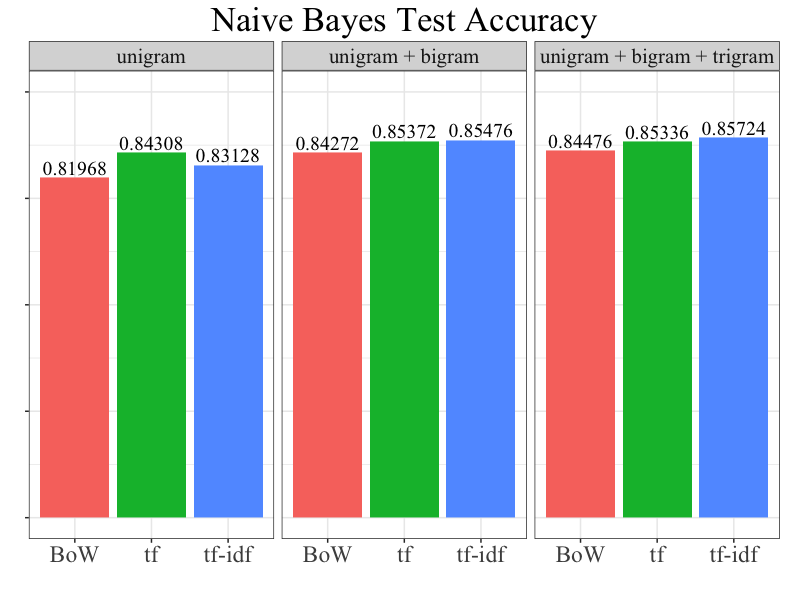
\includegraphics[scale=0.22]{nb.png}
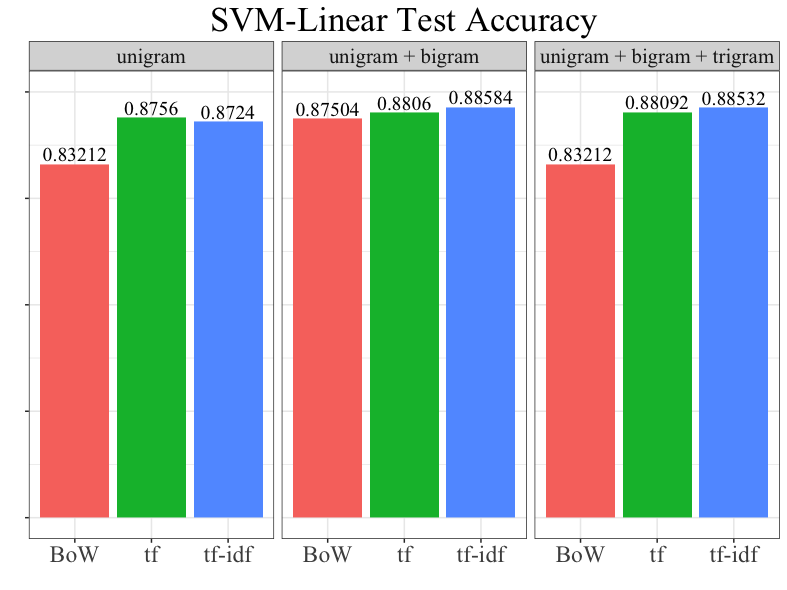
\includegraphics[scale=0.22]{svm.png}
\caption{Baseline Models and Test Accuracy}
\label{fig:a}
\end{figure}


\section{Evaluation of Preliminary Work}

In terms of classifiers, we can see that when using a BoW model, the best test accuracy was given by NB; when using either TF or TF-IDF as feature vectors, the best test accuracy was achieved by linear SVM. The reason why SVM that using RBF kernel performed poorly is because we didn't perform cross-validation during training to select the optimal gamma parameter and used the default value given by the package instead.

In terms of feature vectorization methods, we observed that both TF and TF-IDF give similar results and outperformed BoW model.


\section{Future Work}

In our future work, we hope to first explore feature vectors with richer information such as lexical polarity and part of speech tags. Furthermore, we are interested in finding out how topic modelling could be incorporated into and potentially augment the task of sentiment analysis. Through topic modelling, each document could be learned as a mixture of latent topics in an unsupervised fashion. Inspired by the technique of boosting, random decision forest, and previous works done by Ficamos and Liu \cite{Ficamos}, we think it is reasonable to propose that training classifiers that are specialized in analyzing subsets of reviews discussing similar topics and making a final prediction based on voting would be more effective than training a universal classifier that generalize across the entire dataset. Other than the potential improvement in classification accuracy, since a latent topic is simply a collection of words that could be interpreted and further analyzed, our proposed model also has the merit of being more interpretable in comparison to end-to-end deep learning based models that often learn convoluted feature representations. 


\section{Teammates and Work Division}

 We expect projects done in a group to be more substantial than projects done individually. You should outline what everybody in your group will do and by when each task should be complete.\\
\noindent \textbf{March 11th to March 24th (Feature Vector Improvement)} \\
$\bullet$ More research on ways to improve feature vectors, with a focus on lexical polarity and part of speech tag (Xiangting Chen, Shiqi Xiao) \\
$\bullet$ Test the new feature vectors on the classifier (Linhong Li, Jiachen Ning)\\
$\bullet$  Based on the results from the new feature vectors, make modifications accordingly (All)\\
\textbf{March 25th to April 7th (Topic Modelling)}\\
$\bullet$  Explore topic modelling to identify latent topics (Linhong Li, Jiachen Ning)\\
$\bullet$  Train the classifier and find explanations on why or why not the topic modelling works (Xiangting Chen, Shiqi Xiao) \\
$\bullet$  Start writing final report (All)\\
\textbf{April 8th to April 16th (Poster Preparation)}\\
$\bullet$  Prepare content for the poster (Xiangting Chen, Linhong Li) \\
$\bullet$ Draw result graphs for the poster (Jiachen Ning, Shiqi Xiao) \\
$\bullet$  Create the poster and identify the most important finding from our research project. (All) \\
$\bullet$ Prepare the information we need to convey during the talk that will complement our poster. (All)\\
\textbf{April 17th to May 1st (Final Report)}\\
$\bullet$  Summarize previous results and write the final report (All) 
$\bullet$ Final modification of final report based on the feedbacks from the poster session. (All)

\begin{thebibliography}{99}
\bibitem{Ficamos} Ficamos, P., & Liu, Y. (2016). A topic based approach for sentiment analysis on Twitter data. {\it International Journal of Advanced Computer Science and Applications, 7(12)}, 201-205.
\bibitem{Howard} Howard, J., & Ruder, S. (2018). Universal language model fine-tuning for text classification. arXiv preprint arXiv:1801.06146.
\bibitem{Lin} Lin, C., & He, Y. (2009, November). Joint sentiment/topic model for sentiment analysis. In {\it Proceedings of the 18th ACM conference on Information and knowledge management} (pp. 375-384). ACM.
\bibitem{Mass} Maas, A. L., Daly, R. E., Pham, P. T., Huang, D., Ng, A. Y., & Potts, C. (2011, June). Learning word vectors for sentiment analysis. In {\it Proceedings of the 49th annual meeting of the association for computational linguistics:  Human language technologies-volume 1} (pp.\ 142-150). Association for Computational Linguistics.
\bibitem{Mantyl} M{\"a}ntyl{\"a, M. V., Graziotin, D., & Kuutila, M. (2018). The evolution of sentiment analysis: A review of research topics, venues, and top cited papers. {\it Computer Science Review, 27}, 16-32.
\bibitem{Pang} Pang, B., Lee, L., & Vaithyanathan, S. (2002, July). Thumbs up?: sentiment classification using machine learning techniques. In  {\it Proceedings of the ACL-02 conference on Empirical methods in natural language processing-Volume 10} (pp. 79-86). Association for Computational Linguistics.
\bibitem{Pedregosa} Pedregosa et al. (2011). Scikit-learn: Machine Learning in Python. In {\it Journal of Machine Learning Research 12} (pp. 2825-2830).
\bibitem{Wang} Wang, S., & Manning, C. D. (2012, July). Baselines and bigrams: Simple, good sentiment and topic classification. In {\it Proceedings of the 50th Annual Meeting of the Association for Computational Linguistics: Short Papers-Volume 2 }(pp. 90-94). Association for Computational Linguistics.

  

\end{thebibliography}

\end{document}
